\documentclass[landscape,final,a0paper,fontscale=0.285]{baposter}

\usepackage{calc}
\usepackage{graphicx}
\usepackage{amsmath}
\usepackage{amssymb}
\usepackage{relsize}
\usepackage{multirow}
\usepackage{rotating}
\usepackage{bm}
\usepackage{url}

\usepackage{graphicx}
\usepackage{multicol}

%\usepackage{times}
%\usepackage{helvet}
%\usepackage{bookman}
\usepackage{palatino}

\newcommand{\captionfont}{\footnotesize}

\graphicspath{{images/}{../images/}}
\usetikzlibrary{calc}

\newcommand{\SET}[1]  {\ensuremath{\mathcal{#1}}}
\newcommand{\MAT}[1]  {\ensuremath{\boldsymbol{#1}}}
\newcommand{\VEC}[1]  {\ensuremath{\boldsymbol{#1}}}
\newcommand{\Video}{\SET{V}}
\newcommand{\video}{\VEC{f}}
\newcommand{\track}{x}
\newcommand{\Track}{\SET T}
\newcommand{\LMs}{\SET L}
\newcommand{\lm}{l}
\newcommand{\PosE}{\SET P}
\newcommand{\posE}{\VEC p}
\newcommand{\negE}{\VEC n}
\newcommand{\NegE}{\SET N}
\newcommand{\Occluded}{\SET O}
\newcommand{\occluded}{o}

%%%%%%%%%%%%%%%%%%%%%%%%%%%%%%%%%%%%%%%%%%%%%%%%%%%%%%%%%%%%%%%%%%%%%%%%%%%%%%%%
%%%% Some math symbols used in the text
%%%%%%%%%%%%%%%%%%%%%%%%%%%%%%%%%%%%%%%%%%%%%%%%%%%%%%%%%%%%%%%%%%%%%%%%%%%%%%%%

%%%%%%%%%%%%%%%%%%%%%%%%%%%%%%%%%%%%%%%%%%%%%%%%%%%%%%%%%%%%%%%%%%%%%%%%%%%%%%%%
% Multicol Settings
%%%%%%%%%%%%%%%%%%%%%%%%%%%%%%%%%%%%%%%%%%%%%%%%%%%%%%%%%%%%%%%%%%%%%%%%%%%%%%%%
\setlength{\columnsep}{1.5em}
\setlength{\columnseprule}{0mm}

%%%%%%%%%%%%%%%%%%%%%%%%%%%%%%%%%%%%%%%%%%%%%%%%%%%%%%%%%%%%%%%%%%%%%%%%%%%%%%%%
% Save space in lists. Use this after the opening of the list
%%%%%%%%%%%%%%%%%%%%%%%%%%%%%%%%%%%%%%%%%%%%%%%%%%%%%%%%%%%%%%%%%%%%%%%%%%%%%%%%
\newcommand{\compresslist}{%
\setlength{\itemsep}{1pt}%
\setlength{\parskip}{0pt}%
\setlength{\parsep}{0pt}%
}

%%%%%%%%%%%%%%%%%%%%%%%%%%%%%%%%%%%%%%%%%%%%%%%%%%%%%%%%%%%%%%%%%%%%%%%%%%%%%%
%%% Begin of Document
%%%%%%%%%%%%%%%%%%%%%%%%%%%%%%%%%%%%%%%%%%%%%%%%%%%%%%%%%%%%%%%%%%%%%%%%%%%%%%

\begin{document}

%%%%%%%%%%%%%%%%%%%%%%%%%%%%%%%%%%%%%%%%%%%%%%%%%%%%%%%%%%%%%%%%%%%%%%%%%%%%%%
%%% Here starts the poster
%%%---------------------------------------------------------------------------
%%% Format it to your taste with the options
%%%%%%%%%%%%%%%%%%%%%%%%%%%%%%%%%%%%%%%%%%%%%%%%%%%%%%%%%%%%%%%%%%%%%%%%%%%%%%
% Define some colors

%\definecolor{lightblue}{cmyk}{0.83,0.24,0,0.12}
\definecolor{lightblue}{rgb}{0.145,0.6666,1}

% Draw a video
\newlength{\FSZ}
\newcommand{\drawvideo}[3]{% [0 0.25 0.5 0.75 1 1.25 1.5]
   \noindent\pgfmathsetlength{\FSZ}{\linewidth/#2}
   \begin{tikzpicture}[outer sep=0pt,inner sep=0pt,x=\FSZ,y=\FSZ]
   \draw[color=lightblue!50!black] (0,0) node[outer sep=0pt,inner sep=0pt,text width=\linewidth,minimum height=0] (video) {\noindent#3};
   \path [fill=lightblue!50!black,line width=0pt] 
     (video.north west) rectangle ([yshift=\FSZ] video.north east) 
    \foreach \x in {1,2,...,#2} {
      {[rounded corners=0.6] ($(video.north west)+(-0.7,0.8)+(\x,0)$) rectangle +(0.4,-0.6)}
    }
;
   \path [fill=lightblue!50!black,line width=0pt] 
     ([yshift=-1\FSZ] video.south west) rectangle (video.south east) 
    \foreach \x in {1,2,...,#2} {
      {[rounded corners=0.6] ($(video.south west)+(-0.7,-0.2)+(\x,0)$) rectangle +(0.4,-0.6)}
    }
;
   \foreach \x in {1,...,#1} {
     \draw[color=lightblue!50!black] ([xshift=\x\linewidth/#1] video.north west) -- ([xshift=\x\linewidth/#1] video.south west);
   }
   \foreach \x in {0,#1} {
     \draw[color=lightblue!50!black] ([xshift=\x\linewidth/#1,yshift=1\FSZ] video.north west) -- ([xshift=\x\linewidth/#1,yshift=-1\FSZ] video.south west);
   }
   \end{tikzpicture}
}

\hyphenation{resolution occlusions}
%%
\begin{poster}%
  % Poster Options
  {
  % Show grid to help with alignment
  grid=false,
  % Column spacing
  colspacing=1em,
  % Color style
  bgColorOne=white,
  bgColorTwo=white,
  borderColor=lightblue,
  headerColorOne=black,
  headerColorTwo=lightblue,
  headerFontColor=white,
  boxColorOne=white,
  boxColorTwo=lightblue,
  % Format of textbox
  textborder=roundedleft,
  % Format of text header
  eyecatcher=true,
  headerborder=closed,
  headerheight=0.1\textheight,
%  textfont=\sc, An example of changing the text font
  headershape=roundedright,
  headershade=shadelr,
  headerfont=\Large\bf\textsc, %Sans Serif
  textfont={\setlength{\parindent}{1.5em}},
  boxshade=plain,
%  background=shade-tb,
  background=plain,
  linewidth=2pt
  }
  % Eye Catcher
  {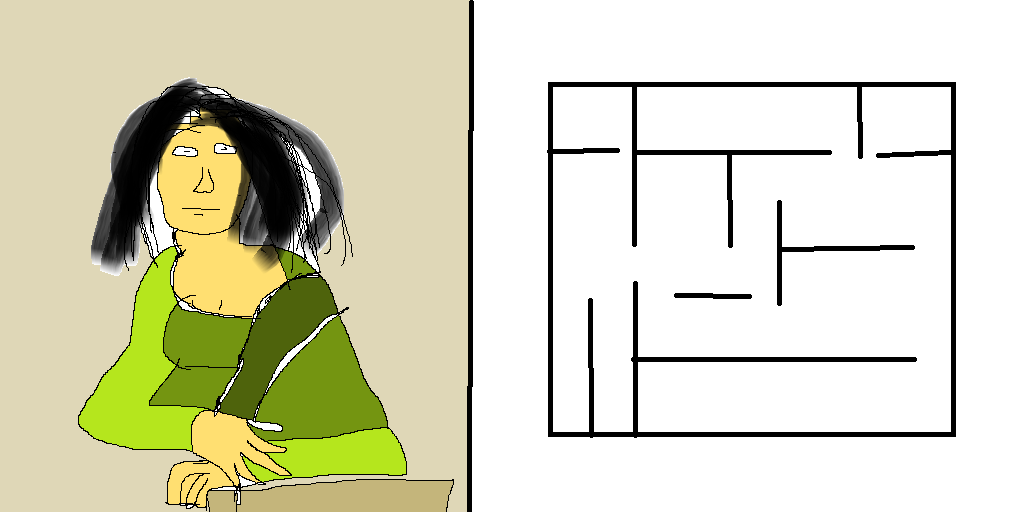
\includegraphics[height=5em]{images/eyecatcher}} 
  % Title
  {\bf\textsc{Procedurally Generating Content from Video Stream}\vspace{0.5em}}
  % Authors
  %{\textsc{\{ Sebastien.Gaulier and Guillaume.Ambrois \}@gmail.com}}
  {\textsc{\ Anonym}}
  % University logo
  {% The makebox allows the title to flow into the logo, this is a hack because of the L shaped logo.
	%
\includegraphics[height=5.0em]{images/logo}
  }

%%%%%%%%%%%%%%%%%%%%%%%%%%%%%%%%%%%%%%%%%%%%%%%%%%%%%%%%%%%%%%%%%%%%%%%%%%%%%%
%%% Now define the boxes that make up the poster
%%%---------------------------------------------------------------------------
%%% Each box has a name and can be placed absolutely or relatively.
%%% The only inconvenience is that you can only specify a relative position 
%%% towards an already declared box. So if you have a box attached to the 
%%% bottom, one to the top and a third one which should be in between, you 
%%% have to specify the top and bottom boxes before you specify the middle 
%%% box.
%%%%%%%%%%%%%%%%%%%%%%%%%%%%%%%%%%%%%%%%%%%%%%%%%%%%%%%%%%%%%%%%%%%%%%%%%%%%%%
    %
    % A coloured circle useful as a bullet with an adjustably strong filling
    \newcommand{\colouredcircle}{%
      \tikz{\useasboundingbox (-0.2em,-0.32em) rectangle(0.2em,0.32em); \draw[draw=black,fill=lightblue,line width=0.03em] (0,0) circle(0.18em);}}

%%%%%%%%%%%%%%%%%%%%%%%%%%%%%%%%%%%%%%%%%%%%%%%%%%%%%%%%%%%%%%%%%%%%%%%%%%%%%%
  \headerbox{Introduction}{name=introduction,column=0,row=0}{
%%%%%%%%%%%%%%%%%%%%%%%%%%%%%%%%%%%%%%%%%%%%%%%%%%%%%%%%%%%%%%%%%%%%%%%%%%%%%%
	 Over the past years, procedurally generated content has become increasingly popular, especially in video games.
	 But the seed (the data used as input for the algorithm) for those procedural algorithms is almost always just a number.
 
	 Meanwhile, computer vision algorithms keep getting faster, stronger and smarter.
 
	 And so we decided to try and mix the two together.
 
	 In this poster, we will explain the design we had in mind, and how we implemented it.
 }

%%%%%%%%%%%%%%%%%%%%%%%%%%%%%%%%%%%%%%%%%%%%%%%%%%%%%%%%%%%%%%%%%%%%%%%%%%%%%%
  \headerbox{Challenge \& Objectives}{name=challenge_objectives,column=1,row=0,bottomaligned=introduction}{
%%%%%%%%%%%%%%%%%%%%%%%%%%%%%%%%%%%%%%%%%%%%%%%%%%%%%%%%%%%%%%%%%%%%%%%%%%%%%%
	We wanted to allow the players to personnalize a bit their experience, by giving them a way to control, even only in a small way, the procedural generation of content.
	 
	The challenge was to find a way for our algorithm to procedurally generate an enjoyable and fun playable level, which the players would feel they have the control on, without giving them total control.
	
	Another challenge was to use OpenCV and Unreal Engine together.
  }

%%%%%%%%%%%%%%%%%%%%%%%%%%%%%%%%%%%%%%%%%%%%%%%%%%%%%%%%%%%%%%%%%%%%%%%%%%%%%%
\headerbox{Results (simplified)}{name=results,column=2,span=2,row=0}{
  %%%%%%%%%%%%%%%%%%%%%%%%%%%%%%%%%%%%%%%%%%%%%%%%%%%%%%%%%%%%%%%%%%%%%%%%%%%%%%
    \drawvideo{5}{40}{%
	    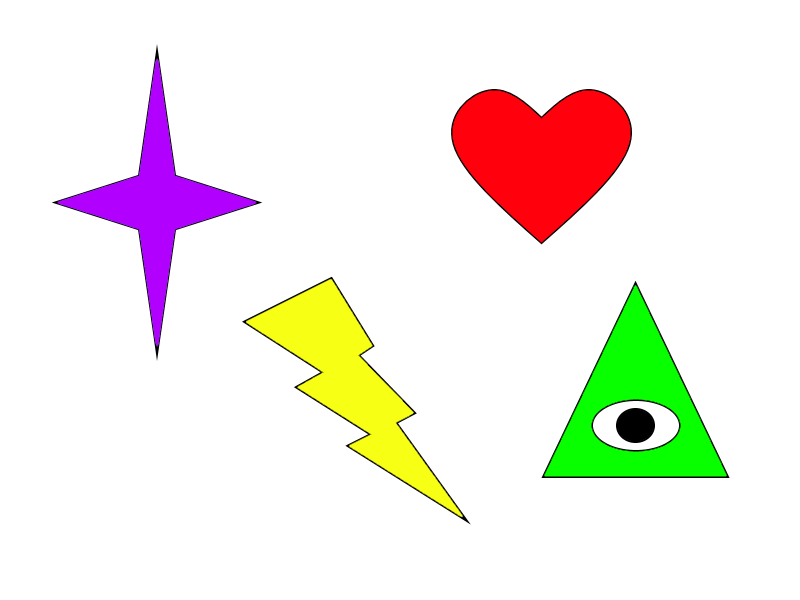
\includegraphics[width=0.2\linewidth]{input_1}%
        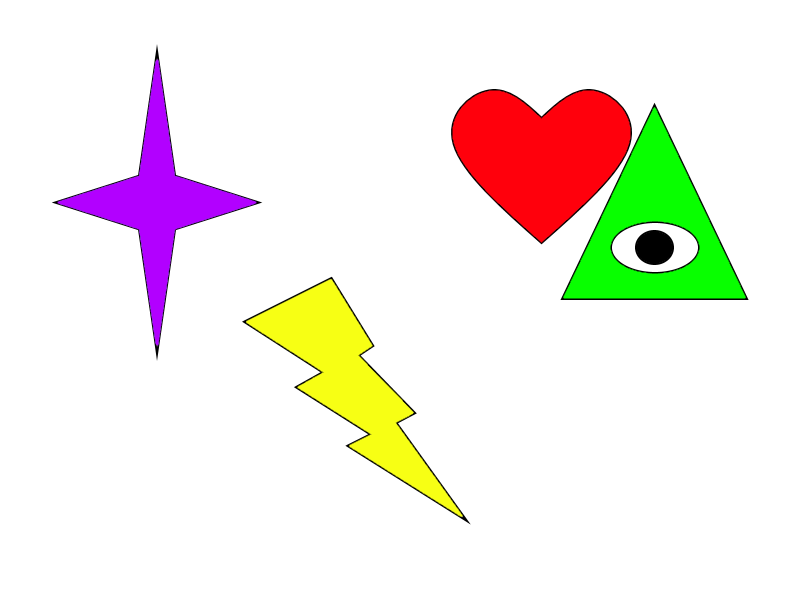
\includegraphics[width=0.2\linewidth]{input_2}%
        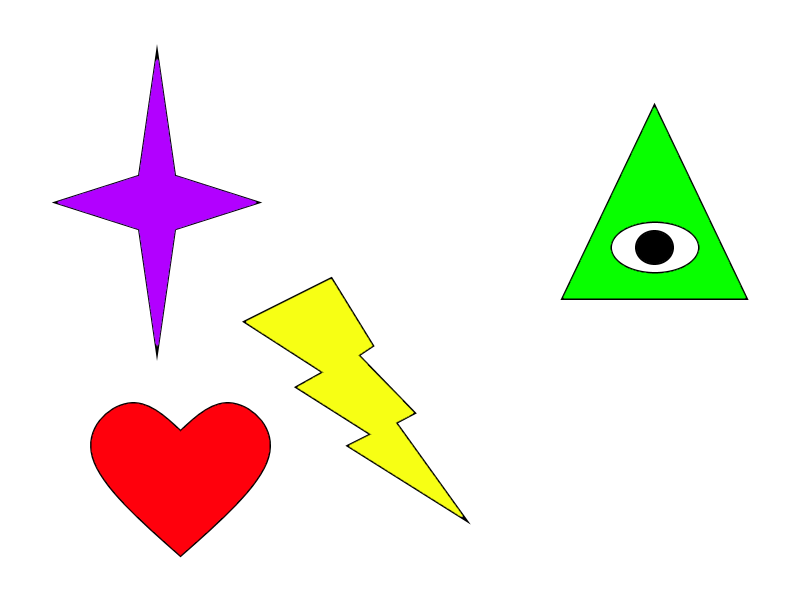
\includegraphics[width=0.2\linewidth]{input_3}%
        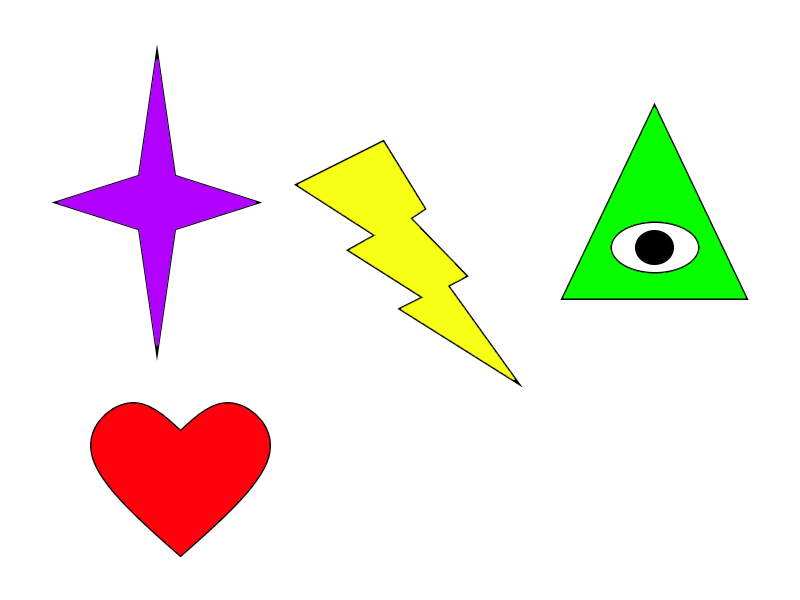
\includegraphics[width=0.2\linewidth]{input_4}%
        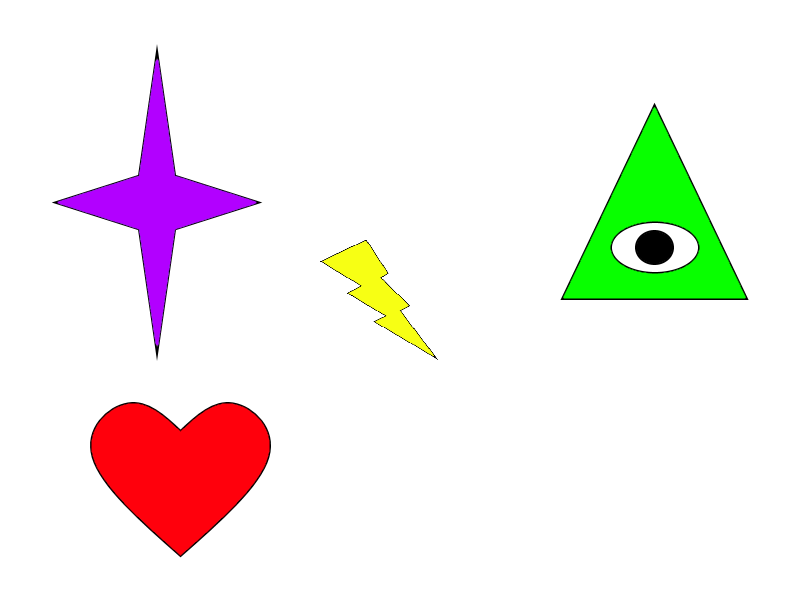
\includegraphics[width=0.2\linewidth]{input_5}%
    }
  \begin{tabular*}{\linewidth}{*{5}{@{}p{0.2\linewidth}@{}}}
    {\hfill{}Frame 1\hfill{}} & 
    {\hfill{}Frame 2\hfill{}} & 
    {\hfill{}Frame 3\hfill{}} &  
    {\hfill{}Frame 4\hfill{}} & 
    {\hfill{}Frame 5\hfill{}}
  \end{tabular*}
  \\[1em]
      \drawvideo{5}{40}{%
          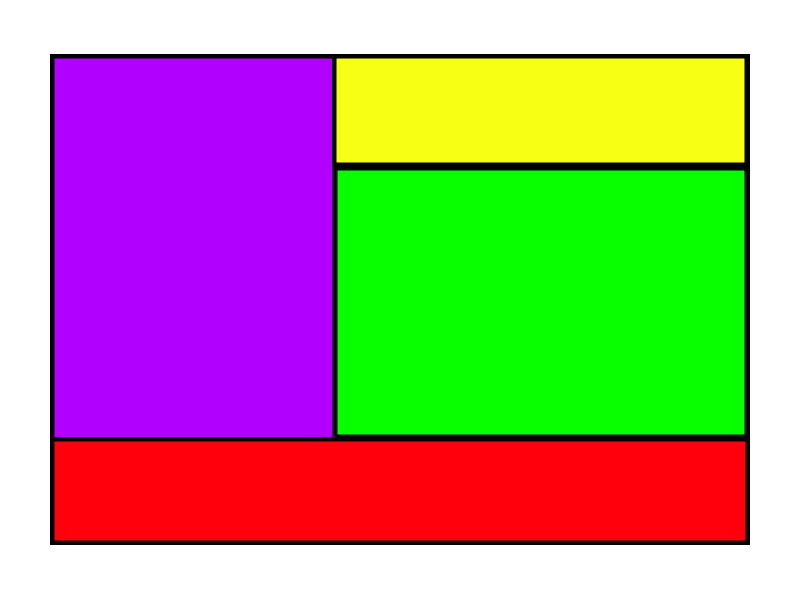
\includegraphics[width=0.2\linewidth]{output_1}%
          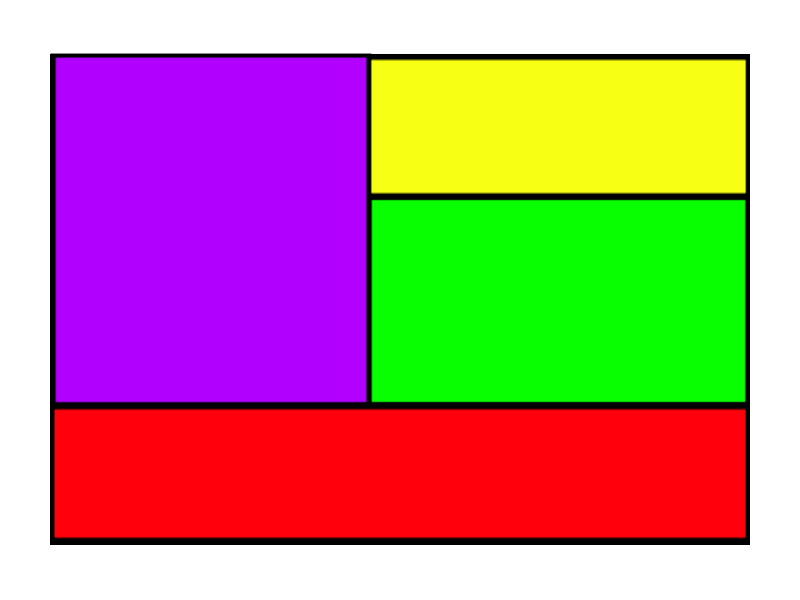
\includegraphics[width=0.2\linewidth]{output_2}%
          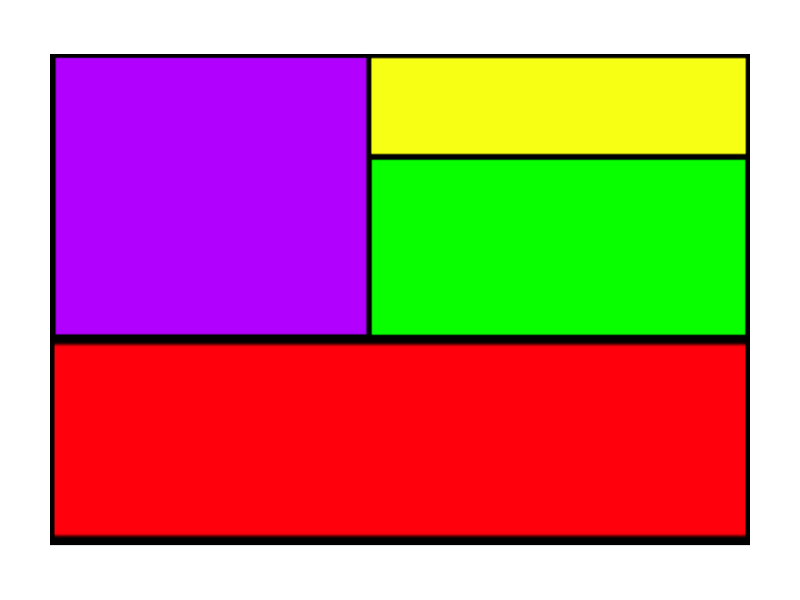
\includegraphics[width=0.2\linewidth]{output_3}%
          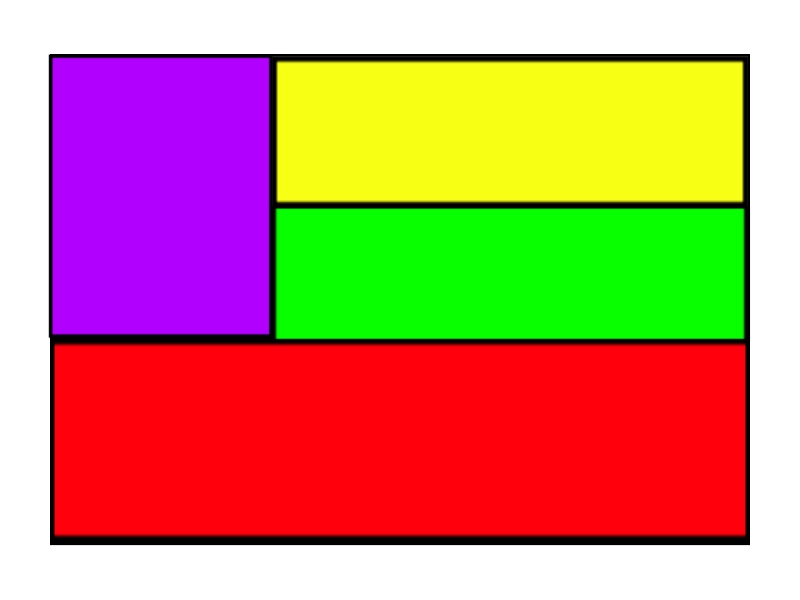
\includegraphics[width=0.2\linewidth]{output_4}%
          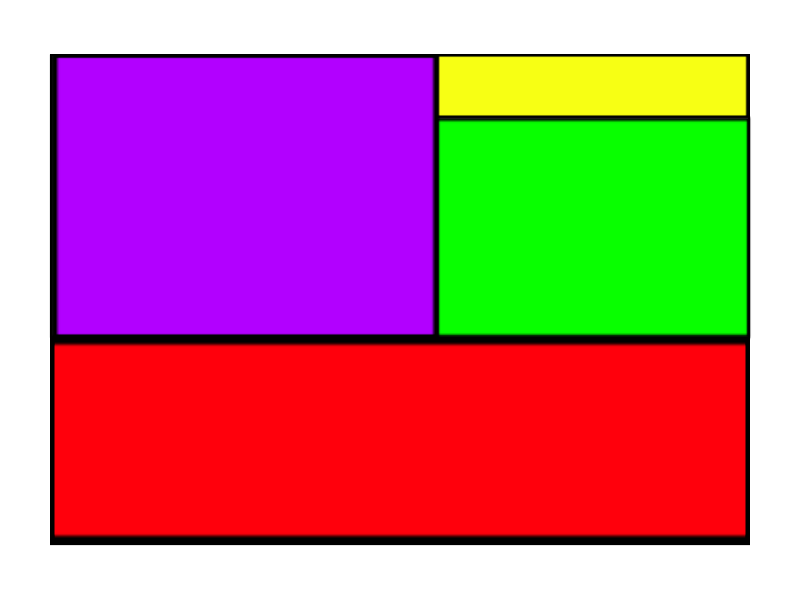
\includegraphics[width=0.2\linewidth]{output_5}%
      }
  \begin{tabular*}{\linewidth}{*{5}{@{}p{0.2\linewidth}@{}}}
    {\hfill{}Frame 1\hfill{}} &
    {\hfill{}Frame 2\hfill{}} &
    {\hfill{}Frame 3\hfill{}} &
    {\hfill{}Frame 4\hfill{}} &
    {\hfill{}Frame 5\hfill{}} 
  \end{tabular*}
      \begin{multicols}{2}
      	Here you can see the input video on the top row ...

		... and the corresponding level on the bottom row.
      \end{multicols}
      \vspace{-0.6em}
}
%%%%%%%%%%%%%%%%%%%%%%%%%%%%%%%%%%%%%%%%%%%%%%%%%%%%%%%%%%%%%%%%%%%%%%%%%%%%%%
  \headerbox{References}{name=references,column=0,span=2,above=bottom}{
%%%%%%%%%%%%%%%%%%%%%%%%%%%%%%%%%%%%%%%%%%%%%%%%%%%%%%%%%%%%%%%%%%%%%%%%%%%%%%
    \smaller
    \bibliographystyle{ieee}
    \renewcommand{\section}[2]{\vskip 0.05em}
      \begin{thebibliography}{1}\itemsep=-0.01em
      \setlength{\baselineskip}{0.4em}
      \bibitem{amberg11:graphtrack}
        B.~Amberg, T. Vetter.
        \newblock {GraphTrack}: {F}ast and {G}lobally {O}ptimal {T}racking in {V}ideos
        \newblock In {\em CVPR '11}
      \bibitem{awf:tracking}
        A.~Buchanan and A.~Fitzgibbon.
        \newblock {I}nteractive {F}eature {T}racking using {K-D} {T}rees and {D}ynamic {P}rogramming.
        \newblock In {\em CVPR '06}
      \end{thebibliography}
   \vspace{0.3em}
  }
%%%%%%%%%%%%%%%%%%%%%%%%%%%%%%%%%%%%%%%%%%%%%%%%%%%%%%%%%%%%%%%%%%%%%%%%%%%%%%
  \headerbox{Improvements}{name=improvements,column=2,span=2,aligned=references,above=bottom}{
%%%%%%%%%%%%%%%%%%%%%%%%%%%%%%%%%%%%%%%%%%%%%%%%%%%%%%%%%%%%%%%%%%%%%%%%%%%%%%
  \begin{multicols}{2}
    Our algorithm could use some optimization, and we plan to allow fine tuning in the future.
    
    We also want to add the possibility to analyze and use the sound in the video.
  \end{multicols}
   \vspace{0.3em}
  }
%%%%%%%%%%%%%%%%%%%%%%%%%%%%%%%%%%%%%%%%%%%%%%%%%%%%%%%%%%%%%%%%%%%%%%%%%%%%%%
 % \headerbox{Source Code}{name=references,column=3,aligned=references,above=bottom}{
%%%%%%%%%%%%%%%%%%%%%%%%%%%%%%%%%%%%%%%%%%%%%%%%%%%%%%%%%%%%%%%%%%%%%%%%%%%%%%
 % The source code can be found at at \\
 % \url{https://github.com/Epono/5A-3DJV-VvVvV_Reloaded}
 %  \vspace{0.3em}
%  }
%%%%%%%%%%%%%%%%%%%%%%%%%%%%%%%%%%%%%%%%%%%%%%%%%%%%%%%%%%%%%%%%%%%%%%%%%%%%%%
\headerbox{Limitations}{name=limitations,column=2,span=2,below=results,above=references}{
  %%%%%%%%%%%%%%%%%%%%%%%%%%%%%%%%%%%%%%%%%%%%%%%%%%%%%%%%%%%%%%%%%%%%%%%%%%%%%%
    \begin{multicols}{2}
		\indent{}For now, our algorithm processes only very simple videos, like simple shapes on a white background, or videos with a fixed camera. This is because tracking elements with a moving camera is much harder than with a fixed camera, and we wanted to focus on refining our procedural algorithm, in order to produce fun levels for the players to play.	
  \\
  \\
  \indent
  \\
  \\
  \indent
  \\
  \\
  \indent   
		Another limitation is the fact that only one player processes the video, others can't participate in the procedural generaion of the level. One way around this issue would be to allow each player to procedurally generate a portion of the level, but this could result in the junctures between each portion being a little off.
		
		Currently, our algorithm doesn't take into account the audio in a video, since we focused on computer vision, but this is something we would really like to add in the next version of our project.	
	\end{multicols}
   \vspace{0.0em}
  }
%%%%%%%%%%%%%%%%%%%%%%%%%%%%%%%%%%%%%%%%%%%%%%%%%%%%%%%%%%%%%%%%%%%%%%%%%%%%%%
  \headerbox{Method}{name=method,column=0,span=2,below=introduction,bottomaligned=limitations}{
%%%%%%%%%%%%%%%%%%%%%%%%%%%%%%%%%%%%%%%%%%%%%%%%%%%%%%%%%%%%%%%%%%%%%%%%%%%%%%
%%\noindent{\centering\includegraphics[width=0.95\linewidth]{images/cluded.pdf}\\}
  In our project, we used Unreal Engine 4 as game engine, and OpenCV 3.1 to process the video from which we want to extract data.
  
  Firstly, for the sake of simplicity, we used short videos (2 to 3 minutes), with a static point of view to get rid of the complexity of keeping track of the camera's movement.
  
  We process each frame of the video, trying to follow the motion of the elements we're tracking. To process these frames we're using contours with OpenCV.
  \\
  \\
  \indent  
  First we need to have a binary image in which your objects should be white and the background should be black.
  
  The OpenCV function FindContours give us a list of the potential object contours we have to analyse in order to filter the shapes we want to draw in our scene.
  
  For that we use the OpenCV ApproxPoly function which return a polygon we have to check whether it's a triangle, a quadrilateral, etc. Then we create a room in our game level which is positionned just like the shape in the original picture.
  
  The shapes identified on each frame are tracked in order to follow their movement, so that we can move the room in the game level too.
  
  So as to track a shape in our frame we can't have multiple objects with the same pattern. We just ignore the polygon if we have already a room like it.
  \\
  \\
  \indent
  Now that we have our shapes we can deal with the color. We are looking for the average color in the pattern to create a specific environment. For that we use the OpenCV mean function with a mask, where the mask is our filled polygon.
  
  With the polygon color extracted we just have to compare with the different type of environment we can create.
  \\
  \\
  \indent
  
   \vspace{0.3em}
  }


\end{poster}

\end{document}
